\documentclass{article}
	\usepackage[margin=1in]{geometry}
	\usepackage[hidelinks, linktoc=all]{hyperref}
	\usepackage{indentfirst}
    \usepackage[russian]{babel}
    \usepackage{subcaption}
   	\usepackage[superscript,biblabel]{cite}
    \usepackage[font=small,labelfont=bf]{caption}
    \usepackage{abstract}
    \usepackage{cleveref}
    \setlength{\parskip}{0.1cm}   
	\setlength{\parindent}{0.7cm}
    \usepackage{graphicx} % Used to insert images
    \usepackage{adjustbox} % Used to constrain images to a maximum size 
   	\usepackage{color} % Allow colors to be defined
    \usepackage{enumerate} % Needed for markdown enumerations to work
    \usepackage{geometry} % Used to adjust the document margins
    \usepackage{amsmath} % Equations
    \usepackage{amssymb} % Equations
    \usepackage[mathletters]{ucs} % Extended unicode (utf-8) support
    \usepackage[utf8x]{inputenc} % Allow utf-8 characters in the tex document
    \usepackage{fancyvrb} % verbatim replacement that allows latex
    \usepackage{grffile} % extends the file name processing of package graphics 
                         % to support a larger range 
    % The hyperref package gives us a pdf with properly built
    % internal navigation ('pdf bookmarks' for the table of contents,
    % internal cross-reference links, web links for URLs, etc.)
    \usepackage{hyperref}
    \usepackage{longtable} % longtable support required by pandoc >1.10
    

	\author{Федоров Глеб, 125}
 	\title{Диплом}

\numberwithin{equation}{section}
\setcounter{tocdepth}{4}
\begin{document}
\maketitle
\tableofcontents
\newpage
\part*{Введение}
\addcontentsline{toc}{part}{Введение}
Квантовый компьютер -- это устройство, хранящее и обрабатывающее информацию в группе квантовых систем, причем обработка информации происходит в результате когерентных взаимодействий систем внутри группы \cite{Lloyd1993}. Каждая квантовая система, как правило, является двухуровневой и носит название ``квантовый бит'' или ``кубит'' (англ. ``qubit'' -- quantum bit). Для осуществления квантового расчета необходимо уметь реализовывать связь между кубитами, управлять состоянием кубитов, сохраняя его чистоту, определять состояние каждого из кубитов в группе и, наконец, изолировать кубиты от окружающей среды, следовательно, в качестве кубитов могут быть использованы любые достаточно изолированные двухуровневые системы, поддающиеся контролю и способные взаимодействовать друг с другом \cite{DiVincenzo1995, DiVincenzo2000, Spiller1996}. В качестве примера можно привести фотоны \cite{Milburn2009}, ионы в ионных ловушках \cite{Cirac1995}, ядерные спины \cite{Kane1998}, атомы в электромагнитных резонаторах\cite{Rempe2008},  электрические системы\cite{Devoret2005} и т.п.

Последние являются одними их самых заманчивых кандидатов на эту роль, если только окажутся подчинены квантовой механике\cite{Devoret1995}. К счастью, явление сверхпроводимости и эффект Джозефсона позволяют наблюдать квантовые эффекты в контурах даже мезоскопического масштаба и создавать так называемые сверхпроводящие (джозефсоновские) кубиты\cite{Clarke2008}. В данной работе проводится исследование одного из них -- потокового сверхпроводящего кубита (впервые предложен в статье\cite{Orlando1999} и назван Flux-кубитом).

Джозефсоновские кубиты имеют два значительных недостатка и одно значительное преимущество в сравнении с микроскопическими кубитами. Первый недостаток касается шума и нарушения чистоты состояния - в силу больших размеров, джозефсоновские кубиты сильнее связываются со средой, что требует дополнительных изысканий в области их изоляции; второй недостаток заключается в том, что в то время как микроскопические кубиты, например, атомы, идентичны друг другу, сверхпроводящие кубиты могут иметь отличия из-за неточностей производства. Для борьбы с этим требуется либо создавать заведомо нечувствительные к дефектам схемы, либо проводить калибровку, в процессе которой параметры цепей измеряются и компенсируются.

Преимущество джозефсоновских кубитов в их гибкости: они могут быть произвольным образом расположены относительно друг друга, а их параметры легко и непрерывно изменяемы в широких пределах. Эта гибкость вместе с некоторыми фундаментальными эффектами\cite{Koch2007} может быть использована для борьбы с первым недостатком, а также предоставляет много вариантов для подстройки параметров, что в значительной степени нивелирует второй недостаток. Далее, накопленный опыт человечества в области изготовления интегральных схем позволит упростить переход к производству реальных устройств, что является очевидным преимуществом в сравнении с другими типами кубитов. Таким образом, скорее всего именно джозефсоновские кубиты и будут применены в первом квантовом компьютере, и именно их следует изучать.

Важно отметить, что сверхпроводящие кубиты могут применяться не только для непосредственного использования в квантовом компьютере, так как по сути являются рукотворными атомами. Они могут быть пригодны для создания метаматериалов \cite{Macha2014}, проведения высокоточных измерений полей\cite{Clarke2006}, использоваться в качестве активной среды\cite{Astafiev2010}, для квантовой криптографии и телепортации \cite{Xia2014} и т.п. 
\newpage
\part{Теоретические сведения}
Данный раздел содержит теоретическое описание явлений, наблюдаемых в экспериментальной части работы. Далее будут кратко рассмотрена теория сверхпроводимости, эффект Джозефсона, затем произведено рассмотрение теории изолированного Flux-кубита, теории его взаимодействия с окружающей средой и, наконец, вопросы измерения и контроля. 
\section{Явление сверхпроводимости}
Сверхпроводимость -- это сложное коллективное явление, свойство некоторых материалов обладать строго нулевым электрическим сопротивлением при достижении ими температуры ниже определенного значения. В настоящий момент доминирующей теорией сверхпроводимости является теория БКШ\cite{Schrieffer1999}, согласно которой электроны в сверхпроводнике при переходе через критическую температуру объединяются в так называемые куперовские пары и претерпевают бозе-конденсацию. Спаривание электронов происходит в результате взаимодействия через фононы, приводящего к эффективному притяжению между ними и образованию связанного состояния на уровне Ферми, отделенного от уровней квазичастичных возбуждений энергетической щелью. Полное описание данного эффекта в рамках микроскопической теории невозможно в данной работе, поэтому мы будем далее пользоваться феноменологической теорией Гинзбурга-Ландау \cite{GL1950}. Сверхпроводящее состояние в рамках этой теории может быть описано параметром порядка или, иначе, модулем так называемой "макроскопической волновой функции куперовских пар":
\begin{equation}
\Psi(\mathbf{r}) = \sqrt{\frac{n_s}{2}}e^{i\theta(\mathbf{r})},
\label{eq:glwf} 
\end{equation}
где $n_s$ -- концентрация сверхпроводящих электронов в сверхпроводнике. Важно подчеркнуть, что она не является настоящей волновой функцией, но тем не менее позволяет получить практически важные результаты. Мы далее считаем, что в изолированном невозмущенном полями сверхпроводнике и модуль, и фаза волновой функции (\ref{eq:glwf}) постоянны.

Из минимизации функционала Гинзбурга-Ландау и одного из уравнений Максвелла можно получить следующее уравнение для сверхпроводящего тока куперовских пар в зависимости от приложенного поля, являющееся обобщением уравнения Лондонов:
\begin{equation}
\mathbf{j}_s = -\frac{i\hbar e}{2m_e}(\Psi^*\nabla\Psi - \Psi\nabla\Psi^*) - \frac{2e^2}{m_e}\mathbf{A}|\Psi|^2.
\label{eq:lond}
\end{equation}
Подставляя сюда $\Psi(\mathbf{r})$ из определения (\ref{eq:glwf}), получим:
\begin{equation}
\mathbf{j}_s = \frac{1}{\Lambda}\left(\frac{\Phi_0}{2\pi}\nabla\theta(\mathbf{r})-\mathbf{A}\right),
\label{eq:lond2}
\end{equation}
где $\displaystyle \Lambda = \frac{m_e}{n_s e^2},\ \Phi_0 = \frac{h}{2e}$. Вторая константа, как будет показано далее, является \textit{квантом магнитного потока}, и имеет важное значение в данной работе.
\section{Эффект Джозефсона}
\subsection{Уравнения Джозефсона}
Эффект Джозефсона\cite{Josephson1964} -- это эффект установления одной макроскопической фазы в двух сверхпроводниках, соединенных через так называемую ``слабую связь''. Слабые связи многообразны: это могут быть тонкие слои диэлектрика, сужения, точечные контакты, прослойки из металла в нормальном состоянии или из ферромагнетика. В случае, если фазы не равны, то через слабую связь будет течь бездиссипативный ток, и будет выполнено некоторое \textit{фазо-токовое соотношение} между током и скачком фазы на переходе. Часто, хотя и не всегда\cite{Golubov2004}, оно оказывается синусоидальным:
\begin{equation}
I_s = I_c \sin(\theta_2 - \theta_1) = I_c \sin\varphi.
\label{eq:CPR}
\end{equation}
Из этой формулы видно, что сверхпроводящий ток $I_s$ не может превысить некоторого значения $I_c$. Это так называемый \textit{критический ток} джозефсоновского перехода, при превышении которого бездиссипативность нарушается, и на переходе устанавливается напряжение V. В этом случае выполнено второе уравнение Джозефсона:
\begin{equation}
\hbar \frac{\partial \varphi}{\partial t} = 2eV,
\label{eq:2JE}
\end{equation}
и наблюдаются осцилляции разности фаз между сверхпроводниками. Величина критического тока рассчитывается из микроскопической теории, например, для перехода SIS верна формула Амбегаокара-Баратова:
\begin{equation}
I_c = \frac{\pi\Delta(T)}{2eR_n}\th\left(\frac{\Delta(T)}{2k_bT}\right),
\label{eq:Ic}
\end{equation}
где через $R_n$ обозначено сопротивление контакта в отсутствие сверхпроводимости, $R_n = \rho\frac{d}{S}$, где $\rho$-удельное сопротивление I-слоя, а $d$ и $S$ - его толщина и площадь.
\subsection{RCSJ-модель}
Для упрощения описания динамики джозефсоновского контакта применяется модель RCSJ (Resistively and Capacitively Shunted Junction), работающая для маленьких переходов со слоем изолятора, когда изменения фазы на размере контакта пренебрежимо малы и присутствует ненулевая геометрическая емкость. 
\begin{figure}[h]
\centering
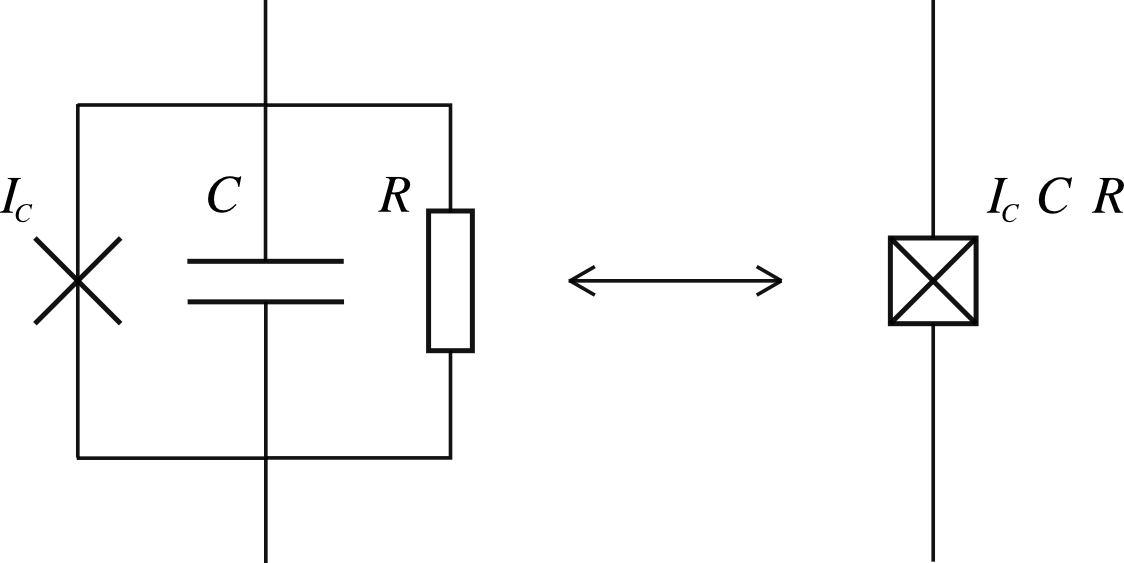
\includegraphics[width=0.5\textwidth]{Pictures/RCSJ.png}
\caption{Схема RCSJ в виде параллельного соединения идеального джозефсоновского перехода с конденсатором и резистором}
\label{fig:RSCJ}
\end{figure}

Принципиальная схема изображена на Рис. \ref{fig:RSCJ}. В случае, когда ток через систему не превышает критического $I_c$, резистор на схеме может быть опущен. В силу параллельности соединения выполнено также соотношение $\displaystyle \frac{\hbar}{2e}\frac{\partial\varphi}{\partial t} = U_C$ между напряжениями на переходе и на конденсаторе, которое устанавливает аналогию между неидеальным переходом и колебательным контуром с нелинейной индуктивностью.

В рамках RCSJ-модели энергия перехода состоит из энергии, запасенной в нелинейной индуктивности идеального перехода, и энергии конденсатора:
\begin{align}
E &= E_{ind}+E_{cap}  \label{eq:JJenrj1}\\
E_{ind} &= \int I_JV_J\, dt = I_c \frac{\hbar}{2e}\int_0^T \sin(\phi(t))\frac{d\phi(t)}{dt}dt \\
&= E_J \int_0^\varphi \sin\phi\, d\phi = E_J [1-\cos\varphi] \notag\\
E_{cap} &= \frac{1}{2}C U_C^2 = \frac{1}{2} C \left(\frac{\Phi_0}{2\pi}\right)^2 \dot \varphi^2 = 
E_C \dot \varphi^2.
\label{eq:JJenrj2}
\end{align}
\subsection{Фазо-потоковое соотношение}
Рассмотрим замкнутый сверхпроводящее кольцо конечной толщины, быть может, прерванный конечным числом джозефсоновских переходов $\{J_1..J_n\}$. Рассмотрим применительно к данному случаю уравнение (\ref{eq:lond2}). Проведем контур $C$ внутри кольца так, чтобы он нигде не приближался к стенкам на расстояние, меньшее глубины проникновения магнитного поля (Рис. \ref{fig:ring}). Тогда сверхток на всей его длине будет равен нулю, и, проинтегрировав по нему (\ref{eq:lond2}), мы получим следующее равенство:
\begin{equation}
\oint\displaylimits_C \mathbf{A}d\mathbf{l} = \frac{\Phi_0}{2\pi}\oint\displaylimits_C \nabla \theta d \mathbf{l} \notag.
\end{equation}
Руководствуясь Рис. \ref{fig:ring}, соображениями однозначности волновой функции (\ref{eq:glwf}) при обходе вокруг контура и теоремой Стокса для $\operatorname{rot} \mathbf{A}$, можем написать:
\begin{align}
\Phi &= \frac{\Phi_0}{2\pi}\left(\sum_i \varphi_n + 2\pi k\right) \notag \\
\sum_i \varphi_n &= 2\pi\left(\frac{\Phi}{\Phi_0} - k\right),\ k\in \mathcal{Z}.
\label{eq:phsflx}
\end{align}

\begin{figure}[h]
\centering
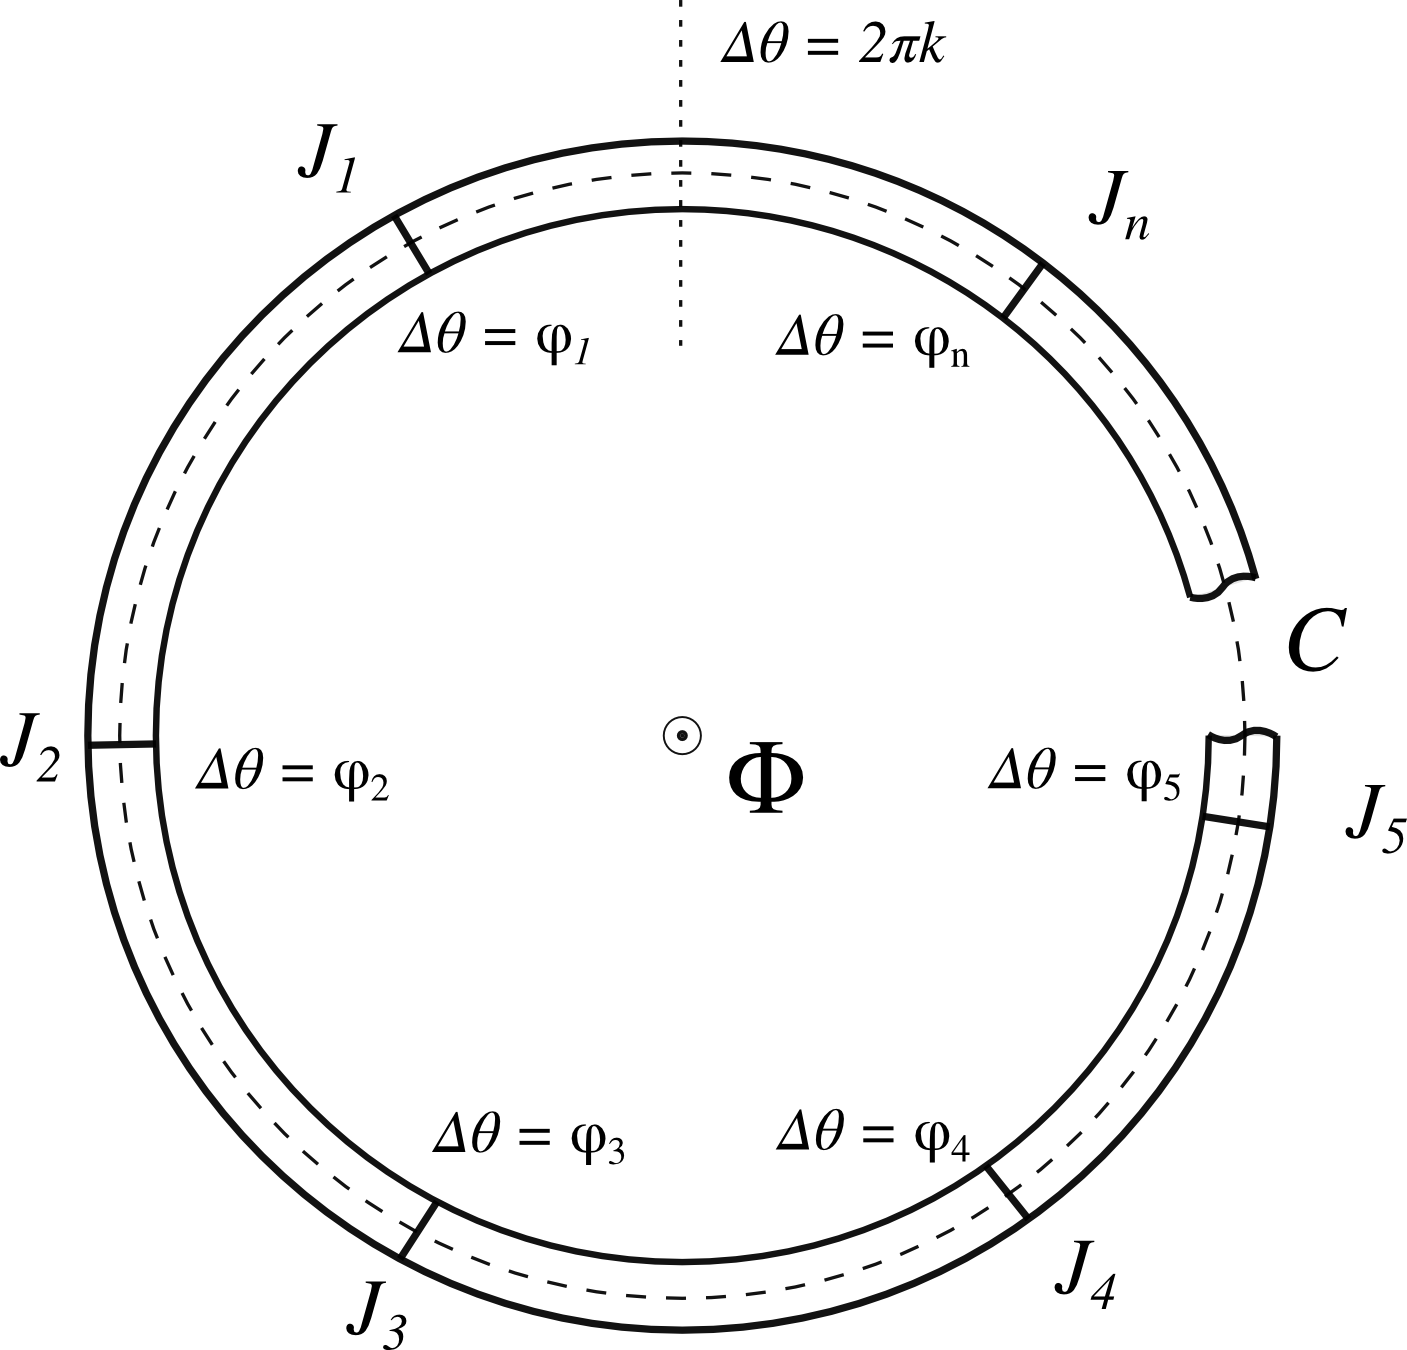
\includegraphics[width=0.4\linewidth]{Pictures/ring.png}
\caption{К выводу фазо-потокового соотношения. Пунктиром обозначен контур интегрирования C. Через $\varphi_i$ обозначены скачки фаз на джозефсоновских контактах, а точками - место разрешенного накопления фазы при полном обходе вокруг кольца $2\pi k,\ k\in\mathcal{Z}$}
\label{fig:ring}
\end{figure}

Таким образом, получено фазо-потоковое соотношение. Видно, что в случае отсутствия в кольце джозефсоновских переходов полученное уравнение (\ref{eq:phsflx}) опишет равенство магнитного потока $\Phi$, проходящего через сверхпроводящее кольцо, целому числу  k квантов потока $\Phi_0$, обосновывая определение этой константы в (\ref{eq:lond2}).


\section{Теория изолированного Flux-кубита}
Flux-кубит, или потоковый трехконтактный сверхпроводящий кубит, был предложен впервые в 1999 году\cite{Orlando1999} и представляет собой сверхпроводящий контур, прерванный в трех местах джозефсоновскими переходами (Рис. \ref{fig:qubit}), два из которых одинаковы, а третий отличается по площади в $\alpha$ раз. Под \textit{изолированным} в данном разделе понимается одиночный кубит, не взаимодействующий с окружением ни диссипативным, ни консервативным образом. Единственным внешним фактором является при таком рассмотрении постоянное магнитное поле, проходящее через контур.

\begin{figure}
\centering
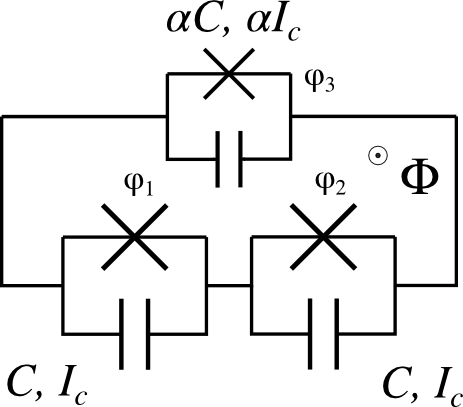
\includegraphics[width=0.4\textwidth]{Pictures/qubit}
\caption{Принципиальная схема Flux-кубита в рамках RSCJ-модели. Два из трех переходов по площади одинаковы, площадь третьего по сравнению с ними в $\alpha$ раз отличается (параметры отличаются в то же число раз согласно формулам для емкости конденсатора и (\ref{eq:Ic})). $\Phi$ -- поток, пронизывающий контур. Резисторы не изображены, так как рабочий ток переходов меньше $I_c$}
\label{fig:qubit}
\end{figure}

\subsection{Построение гамильтониана}
Для того, чтобы провести квантово-механическое рассмотрение кубита, требуется записать его гамильтониан. Для этого прежде всего нужно понять, какими независимыми степенями свободы он обладает. Вообще говоря, состояние одиночного джозефсоновского перехода, в силу того, что в параллельном соединении RCSJ-модели $U = \frac{\hbar}{2e}\dot\varphi$, целиком описывается своей разностью фаз. Для трех невзаимодействующих переходов таких разностей будет три, и их и следует выбрать в качестве обобщенных координат системы. Однако в случае замкнутого контура дополнительно накладывается фазо-потоковое соотношение (\ref{eq:phsflx}):
\begin{equation}
\varphi_1 + \varphi_2 + \varphi_3 = 2\pi\left(\frac{\Phi}{\Phi_0} - k\right),\ k\in \mathcal{Z}.
\label{eq:qubit_phsflx}
\end{equation}
Таким образом, в контуре на Рис. \ref{fig:qubit} остаются независимыми только две разности фаз из трех. Введя их в качестве обобщенных координат, можно понять, что является аналогом кинетической, а что -- потенциальной энергии системы. В уравнениях (\ref{eq:JJenrj1})-(\ref{eq:JJenrj2}) энергия перехода зависит непосредственно от $\varphi$, а емкостная от $\dot \varphi$. Таким образом, переход запасает потенциальную, а емкость кинетическую энергию. Энергия магнитного поля, возникающего при течении тока в кольце, считается малой в силу малости геометрической индуктивности кубита по сравнению с джозефсоновской индуктивностью переходов\cite{Orlando1999}. Теперь можно записать лагранжиан системы, используя все те же уравнения (\ref{eq:JJenrj1})-(\ref{eq:JJenrj2}) и выражая разность фаз $\varphi_3$ отличающегося перехода через разности фаз $\varphi_1$ и $\varphi_2$ одинаковых переходов при помощи (\ref{eq:qubit_phsflx}):
\begin{align*}
\mathcal{L} &= \mathcal{T}-\mathcal{U}, \\
\mathcal{T} &= E_C =\frac{1}{2}\sum_{i=1}^3 C_i V_i^2 = \frac{1}{2} \left(\frac{\Phi_0}{2\pi}\right)^2 \left[C(\dot \varphi_1)^2 + \alpha C \left(\dot \varphi_1 + \dot\varphi_2\right)^2 + C(\dot \varphi_2)^2\right] \notag \\
&= \frac{1}{2}\left(\frac{\Phi_0}{2\pi}\right)^2 \vec{\dot \varphi}^T C \left(\begin{matrix}
1+\alpha & \alpha \\
\alpha & 1+\alpha
\end{matrix}
\right)
\vec{\dot \varphi},\ \vec{\dot\varphi} = \left(\begin{matrix}
\dot\varphi_1 \\
\dot\varphi_2
\end{matrix}\right), \\
\mathcal{U} &= E_J\left[2+\alpha + \cos\varphi_1 + \cos\varphi_2 + \alpha \cos\left(2\pi\frac{\Phi}{\Phi_0} - \varphi_1 - \varphi_2 \right)\right].
\end{align*}
Строить гамильтониан системы из такого лагранжиана не очень удобно, поэтому предварительно произведем замену координат $\displaystyle \phi = \frac{\varphi_1 + \varphi_2}{2},\ \theta = \frac{\varphi_1 - \varphi_2}{2}$:
\begin{align*}
\mathcal{T} & \overset {\varphi_1, \varphi_2 \rightarrow \phi, \theta}{=}
C\left(\frac{\Phi_0}{2\pi}\right)^2 (\begin{matrix}
\dot \phi & \dot \theta
\end{matrix})
\left(\begin{matrix}
1+2\alpha & 0\\
0 & 1
\end{matrix}
\right)
\left(\begin{matrix}
\dot \phi \\ \dot \theta
\end{matrix}\right), \\
\mathcal{U} &\overset {\varphi_1, \varphi_2 \rightarrow \phi, \theta}{=} E_J\left[2+\alpha - 2\cos(\phi)\cos(\theta) - \alpha\cos\left(2\pi\frac{\Phi}{\Phi_0} -2\phi\right)\right].
\end{align*}
Теперь, стандартным образом вводя обобщенный импульс 
$\displaystyle \vec p = \left(\begin{matrix}p_\phi\\p_\theta\end{matrix}\right) = \left(\begin{matrix}\frac{\partial\mathcal{L}}{\partial\dot\phi}\\\frac{\partial\mathcal{L}}{\partial\dot\theta}\end{matrix}\right)$ и производя преобразование Лежандра, получим итоговый гамильтониан системы:
\begin{align*}
\mathcal{H} = \frac{p_\phi^2}{2M_\phi} &+ \frac{p_\theta^2}{2M_\theta}+ E_J\left[2+\alpha - 2\cos(\phi)\cos(\theta) - \alpha\cos\left(2\pi\frac{\Phi}{\Phi_0} -2\phi\right)\right], \\
M_\phi &= 2C\left(\frac{\Phi_0}{2\pi}\right)^2(1+2\alpha),\ M_\theta = 2C\left(\frac{\Phi_0}{2\pi}\right)^2.
\end{align*}
Далее, осуществляя переход к операторному виду квантовой механики, можно получить оператор Гамильтона для сверхпроводящего потокового кубита в терминах исключительно $E_C$ и $E_J$:
\begin{align}
\hat{\mathcal{H}} = E_C\left[-\frac{2}{1 + 2\alpha}\frac{\partial^2}{\partial\phi^2} 
- 2\frac{\partial^2}{\partial\theta^2}\right]+ E_J\left[2+\alpha - 2\cos(\phi)\cos(\theta) - \alpha\cos\left(2\pi\frac{\Phi}{\Phi_0} -2\phi \right)\right].
\end{align}



\newpage
\part{Экспериментальная часть}
\part{Результаты}
\part{Заключение}

\bibliographystyle{ugost2008}
\bibliography{Thesis.bib}

\end{document}